\documentclass[12pt]{article}

%packages
%\usepackage{latexsym}
\usepackage{graphicx}
\usepackage{color}
\usepackage{amsmath}
\usepackage{dsfont}
\usepackage{placeins}
\usepackage{amssymb}
\usepackage{wasysym}
\usepackage{abstract}
\usepackage{hyperref}
\usepackage{etoolbox}
\usepackage{datetime}
\usepackage{xcolor}
\settimeformat{ampmtime}

%\usepackage{pstricks,pst-node,pst-tree}

%\usepackage{algpseudocode}
%\usepackage{amsthm}
%\usepackage{hyperref}
%\usepackage{mathrsfs}
%\usepackage{amsfonts}
%\usepackage{bbding}
%\usepackage{listings}
%\usepackage{appendix}
\usepackage[margin=1in]{geometry}
%\geometry{papersize={8.5in,11in},total={6.5in,9in}}
%\usepackage{cancel}
%\usepackage{algorithmic, algorithm}

\makeatletter
\def\maxwidth{ %
  \ifdim\Gin@nat@width>\linewidth
    \linewidth
  \else
    \Gin@nat@width
  \fi
}
\makeatother

\definecolor{fgcolor}{rgb}{0.345, 0.345, 0.345}
\newcommand{\hlnum}[1]{\textcolor[rgb]{0.686,0.059,0.569}{#1}}%
\newcommand{\hlstr}[1]{\textcolor[rgb]{0.192,0.494,0.8}{#1}}%
\newcommand{\hlcom}[1]{\textcolor[rgb]{0.678,0.584,0.686}{\textit{#1}}}%
\newcommand{\hlopt}[1]{\textcolor[rgb]{0,0,0}{#1}}%
\newcommand{\hlstd}[1]{\textcolor[rgb]{0.345,0.345,0.345}{#1}}%
\newcommand{\hlkwa}[1]{\textcolor[rgb]{0.161,0.373,0.58}{\textbf{#1}}}%
\newcommand{\hlkwb}[1]{\textcolor[rgb]{0.69,0.353,0.396}{#1}}%
\newcommand{\hlkwc}[1]{\textcolor[rgb]{0.333,0.667,0.333}{#1}}%
\newcommand{\hlkwd}[1]{\textcolor[rgb]{0.737,0.353,0.396}{\textbf{#1}}}%

\usepackage{framed}
\makeatletter
\newenvironment{kframe}{%
 \def\at@end@of@kframe{}%
 \ifinner\ifhmode%
  \def\at@end@of@kframe{\end{minipage}}%
  \begin{minipage}{\columnwidth}%
 \fi\fi%
 \def\FrameCommand##1{\hskip\@totalleftmargin \hskip-\fboxsep
 \colorbox{shadecolor}{##1}\hskip-\fboxsep
     % There is no \\@totalrightmargin, so:
     \hskip-\linewidth \hskip-\@totalleftmargin \hskip\columnwidth}%
 \MakeFramed {\advance\hsize-\width
   \@totalleftmargin\z@ \linewidth\hsize
   \@setminipage}}%
 {\par\unskip\endMakeFramed%
 \at@end@of@kframe}
\makeatother

\definecolor{shadecolor}{rgb}{.77, .77, .77}
\definecolor{messagecolor}{rgb}{0, 0, 0}
\definecolor{warningcolor}{rgb}{1, 0, 1}
\definecolor{errorcolor}{rgb}{1, 0, 0}
\newenvironment{knitrout}{}{} % an empty environment to be redefined in TeX

\usepackage{alltt}
\usepackage[T1]{fontenc}

\newcommand{\qu}[1]{``#1''}
\newcounter{probnum}
\setcounter{probnum}{1}

%create definition to allow local margin changes
\def\changemargin#1#2{\list{}{\rightmargin#2\leftmargin#1}\item[]}
\let\endchangemargin=\endlist 

%allow equations to span multiple pages
\allowdisplaybreaks

%define colors and color typesetting conveniences
\definecolor{gray}{rgb}{0.5,0.5,0.5}
\definecolor{black}{rgb}{0,0,0}
\definecolor{white}{rgb}{1,1,1}
\definecolor{blue}{rgb}{0.5,0.5,1}
\newcommand{\inblue}[1]{\color{blue}#1 \color{black}}
\definecolor{green}{rgb}{0.133,0.545,0.133}
\newcommand{\ingreen}[1]{\color{green}#1 \color{black}}
\definecolor{yellow}{rgb}{1,1,0}
\newcommand{\inyellow}[1]{\color{yellow}#1 \color{black}}
\definecolor{orange}{rgb}{0.9,0.649,0}
\newcommand{\inorange}[1]{\color{orange}#1 \color{black}}
\definecolor{red}{rgb}{1,0.133,0.133}
\newcommand{\inred}[1]{\color{red}#1 \color{black}}
\definecolor{purple}{rgb}{0.58,0,0.827}
\newcommand{\inpurple}[1]{\color{purple}#1 \color{black}}
\definecolor{backgcode}{rgb}{0.97,0.97,0.8}
\definecolor{Brown}{cmyk}{0,0.81,1,0.60}
\definecolor{OliveGreen}{cmyk}{0.64,0,0.95,0.40}
\definecolor{CadetBlue}{cmyk}{0.62,0.57,0.23,0}

%define new math operators
\DeclareMathOperator*{\argmax}{arg\,max~}
\DeclareMathOperator*{\argmin}{arg\,min~}
\DeclareMathOperator*{\argsup}{arg\,sup~}
\DeclareMathOperator*{\arginf}{arg\,inf~}
\DeclareMathOperator*{\convolution}{\text{\Huge{$\ast$}}}
\newcommand{\infconv}[2]{\convolution^\infty_{#1 = 1} #2}
%true functions

%%%% GENERAL SHORTCUTS

%shortcuts for pure typesetting conveniences
\newcommand{\bv}[1]{\boldsymbol{#1}}

%shortcuts for compound constants
\newcommand{\BetaDistrConst}{\dfrac{\Gamma(\alpha + \beta)}{\Gamma(\alpha)\Gamma(\beta)}}
\newcommand{\NormDistrConst}{\dfrac{1}{\sqrt{2\pi\sigma^2}}}

%shortcuts for conventional symbols
\newcommand{\tsq}{\tau^2}
\newcommand{\tsqh}{\hat{\tau}^2}
\newcommand{\sigsq}{\sigma^2}
\newcommand{\sigsqsq}{\parens{\sigma^2}^2}
\newcommand{\sigsqovern}{\dfrac{\sigsq}{n}}
\newcommand{\tausq}{\tau^2}
\newcommand{\tausqalpha}{\tau^2_\alpha}
\newcommand{\tausqbeta}{\tau^2_\beta}
\newcommand{\tausqsigma}{\tau^2_\sigma}
\newcommand{\betasq}{\beta^2}
\newcommand{\sigsqvec}{\bv{\sigma}^2}
\newcommand{\sigsqhat}{\hat{\sigma}^2}
\newcommand{\sigsqhatmlebayes}{\sigsqhat_{\text{Bayes, MLE}}}
\newcommand{\sigsqhatmle}[1]{\sigsqhat_{#1, \text{MLE}}}
\newcommand{\bSigma}{\bv{\Sigma}}
\newcommand{\bSigmainv}{\bSigma^{-1}}
\newcommand{\thetavec}{\bv{\theta}}
\newcommand{\thetahat}{\hat{\theta}}
\newcommand{\thetahatmle}{\hat{\theta}_{\mathrm{MLE}}}
\newcommand{\thetavechatmle}{\hat{\thetavec}_{\mathrm{MLE}}}
\newcommand{\muhat}{\hat{\mu}}
\newcommand{\musq}{\mu^2}
\newcommand{\muvec}{\bv{\mu}}
\newcommand{\muhatmle}{\muhat_{\text{MLE}}}
\newcommand{\lambdahat}{\hat{\lambda}}
\newcommand{\lambdahatmle}{\lambdahat_{\text{MLE}}}
\newcommand{\etavec}{\bv{\eta}}
\newcommand{\alphavec}{\bv{\alpha}}
\newcommand{\minimaxdec}{\delta^*_{\mathrm{mm}}}
\newcommand{\ybar}{\bar{y}}
\newcommand{\xbar}{\bar{x}}
\newcommand{\iid}{~{\buildrel iid \over \sim}~}
\newcommand{\inddist}{~{\buildrel ind \over \sim}~}
\newcommand{\approxdist}{~{\buildrel approx \over \sim}~}
\newcommand{\equalsindist}{~{\buildrel d \over =}~}
\newcommand{\loglik}[1]{\ell\parens{#1}}
\newcommand{\thetahatkminone}{\thetahat^{(k-1)}}
\newcommand{\thetahatkplusone}{\thetahat^{(k+1)}}
\newcommand{\thetahatk}{\thetahat^{(k)}}
\newcommand{\half}{\frac{1}{2}}
\newcommand{\third}{\frac{1}{3}}
\newcommand{\twothirds}{\frac{2}{3}}
\newcommand{\fourth}{\frac{1}{4}}
\newcommand{\fifth}{\frac{1}{5}}
\newcommand{\sixth}{\frac{1}{6}}

%shortcuts for vector and matrix notation
\newcommand{\A}{\bv{A}}
\newcommand{\At}{\A^T}
\newcommand{\Ainv}{\inverse{\A}}
\newcommand{\B}{\bv{B}}
\newcommand{\K}{\bv{K}}
\newcommand{\Kt}{\K^T}
\newcommand{\Kinv}{\inverse{K}}
\newcommand{\Kinvt}{(\Kinv)^T}
\newcommand{\M}{\bv{M}}
\newcommand{\Bt}{\B^T}
\newcommand{\Q}{\bv{Q}}
\newcommand{\Qt}{\Q^T}
\newcommand{\R}{\bv{R}}
\newcommand{\Rt}{\R^T}
\newcommand{\Z}{\bv{Z}}
\newcommand{\X}{\bv{X}}
\newcommand{\Xsub}{\X_{\text{(sub)}}}
\newcommand{\Xsubadj}{\X_{\text{(sub,adj)}}}
\newcommand{\I}{\bv{I}}
\newcommand{\Y}{\bv{Y}}
\newcommand{\sigsqI}{\sigsq\I}
\renewcommand{\P}{\bv{P}}
\newcommand{\Psub}{\P_{\text{(sub)}}}
\newcommand{\Pt}{\P^T}
\newcommand{\Pii}{P_{ii}}
\newcommand{\Pij}{P_{ij}}
\newcommand{\IminP}{(\I-\P)}
\newcommand{\Xt}{\bv{X}^T}
\newcommand{\XtX}{\Xt\X}
\newcommand{\XtXinv}{\parens{\Xt\X}^{-1}}
\newcommand{\XtXinvXt}{\XtXinv\Xt}
\newcommand{\XXtXinvXt}{\X\XtXinvXt}
\newcommand{\x}{\bv{x}}
\newcommand{\onevec}{\bv{1}}
\newcommand{\oneton}{1, \ldots, n}
\newcommand{\yoneton}{y_1, \ldots, y_n}
\newcommand{\yonetonorder}{y_{(1)}, \ldots, y_{(n)}}
\newcommand{\Yoneton}{Y_1, \ldots, Y_n}
\newcommand{\iinoneton}{i \in \braces{\oneton}}
\newcommand{\onetom}{1, \ldots, m}
\newcommand{\jinonetom}{j \in \braces{\onetom}}
\newcommand{\xoneton}{x_1, \ldots, x_n}
\newcommand{\Xoneton}{X_1, \ldots, X_n}
\newcommand{\xt}{\x^T}
\newcommand{\y}{\bv{y}}
\newcommand{\yt}{\y^T}
\renewcommand{\c}{\bv{c}}
\newcommand{\ct}{\c^T}
\newcommand{\tstar}{\bv{t}^*}
\renewcommand{\u}{\bv{u}}
\renewcommand{\v}{\bv{v}}
\renewcommand{\a}{\bv{a}}
\newcommand{\s}{\bv{s}}
\newcommand{\yadj}{\y_{\text{(adj)}}}
\newcommand{\xjadj}{\x_{j\text{(adj)}}}
\newcommand{\xjadjM}{\x_{j \perp M}}
\newcommand{\yhat}{\hat{\y}}
\newcommand{\yhatsub}{\yhat_{\text{(sub)}}}
\newcommand{\yhatstar}{\yhat^*}
\newcommand{\yhatstarnew}{\yhatstar_{\text{new}}}
\newcommand{\z}{\bv{z}}
\newcommand{\zt}{\z^T}
\newcommand{\bb}{\bv{b}}
\newcommand{\bbt}{\bb^T}
\newcommand{\bbeta}{\bv{\beta}}
\newcommand{\beps}{\bv{\epsilon}}
\newcommand{\bepst}{\beps^T}
\newcommand{\e}{\bv{e}}
\newcommand{\Mofy}{\M(\y)}
\newcommand{\KofAlpha}{K(\alpha)}
\newcommand{\ellset}{\mathcal{L}}
\newcommand{\oneminalph}{1-\alpha}
\newcommand{\SSE}{\text{SSE}}
\newcommand{\SSEsub}{\text{SSE}_{\text{(sub)}}}
\newcommand{\MSE}{\text{MSE}}
\newcommand{\RMSE}{\text{RMSE}}
\newcommand{\SSR}{\text{SSR}}
\newcommand{\SST}{\text{SST}}
\newcommand{\JSest}{\delta_{\text{JS}}(\x)}
\newcommand{\Bayesest}{\delta_{\text{Bayes}}(\x)}
\newcommand{\EmpBayesest}{\delta_{\text{EmpBayes}}(\x)}
\newcommand{\BLUPest}{\delta_{\text{BLUP}}}
\newcommand{\MLEest}[1]{\hat{#1}_{\text{MLE}}}

%shortcuts for Linear Algebra stuff (i.e. vectors and matrices)
\newcommand{\twovec}[2]{\bracks{\begin{array}{c} #1 \\ #2 \end{array}}}
\newcommand{\threevec}[3]{\bracks{\begin{array}{c} #1 \\ #2 \\ #3 \end{array}}}
\newcommand{\fivevec}[5]{\bracks{\begin{array}{c} #1 \\ #2 \\ #3 \\ #4 \\ #5 \end{array}}}
\newcommand{\twobytwomat}[4]{\bracks{\begin{array}{cc} #1 & #2 \\ #3 & #4 \end{array}}}
\newcommand{\threebytwomat}[6]{\bracks{\begin{array}{cc} #1 & #2 \\ #3 & #4 \\ #5 & #6 \end{array}}}

%shortcuts for conventional compound symbols
\newcommand{\thetainthetas}{\theta \in \Theta}
\newcommand{\reals}{\mathbb{R}}
\newcommand{\complexes}{\mathbb{C}}
\newcommand{\rationals}{\mathbb{Q}}
\newcommand{\integers}{\mathbb{Z}}
\newcommand{\naturals}{\mathbb{N}}
\newcommand{\forallninN}{~~\forall n \in \naturals}
\newcommand{\forallxinN}[1]{~~\forall #1 \in \reals}
\newcommand{\matrixdims}[2]{\in \reals^{\,#1 \times #2}}
\newcommand{\inRn}[1]{\in \reals^{\,#1}}
\newcommand{\mathimplies}{\quad\Rightarrow\quad}
\newcommand{\mathlogicequiv}{\quad\Leftrightarrow\quad}
\newcommand{\eqncomment}[1]{\quad \text{(#1)}}
\newcommand{\limitn}{\lim_{n \rightarrow \infty}}
\newcommand{\limitN}{\lim_{N \rightarrow \infty}}
\newcommand{\limitd}{\lim_{d \rightarrow \infty}}
\newcommand{\limitt}{\lim_{t \rightarrow \infty}}
\newcommand{\limitsupn}{\limsup_{n \rightarrow \infty}~}
\newcommand{\limitinfn}{\liminf_{n \rightarrow \infty}~}
\newcommand{\limitk}{\lim_{k \rightarrow \infty}}
\newcommand{\limsupn}{\limsup_{n \rightarrow \infty}}
\newcommand{\limsupk}{\limsup_{k \rightarrow \infty}}
\newcommand{\floor}[1]{\left\lfloor #1 \right\rfloor}
\newcommand{\ceil}[1]{\left\lceil #1 \right\rceil}

%shortcuts for environments
\newcommand{\beqn}{\vspace{-0.25cm}\begin{eqnarray*}}
\newcommand{\eeqn}{\end{eqnarray*}}
\newcommand{\bneqn}{\vspace{-0.25cm}\begin{eqnarray}}
\newcommand{\eneqn}{\end{eqnarray}}

%shortcuts for mini environments
\newcommand{\parens}[1]{\left(#1\right)}
\newcommand{\squared}[1]{\parens{#1}^2}
\newcommand{\tothepow}[2]{\parens{#1}^{#2}}
\newcommand{\prob}[1]{\mathbb{P}\parens{#1}}
\newcommand{\cprob}[2]{\prob{#1~|~#2}}
\newcommand{\littleo}[1]{o\parens{#1}}
\newcommand{\bigo}[1]{O\parens{#1}}
\newcommand{\Lp}[1]{\mathbb{L}^{#1}}
\renewcommand{\arcsin}[1]{\text{arcsin}\parens{#1}}
\newcommand{\prodonen}[2]{\bracks{\prod_{#1=1}^n #2}}
\newcommand{\mysum}[4]{\sum_{#1=#2}^{#3} #4}
\newcommand{\sumonen}[2]{\sum_{#1=1}^n #2}
\newcommand{\infsum}[2]{\sum_{#1=1}^\infty #2}
\newcommand{\infprod}[2]{\prod_{#1=1}^\infty #2}
\newcommand{\infunion}[2]{\bigcup_{#1=1}^\infty #2}
\newcommand{\infinter}[2]{\bigcap_{#1=1}^\infty #2}
\newcommand{\infintegral}[2]{\int^\infty_{-\infty} #2 ~\text{d}#1}
\newcommand{\supthetas}[1]{\sup_{\thetainthetas}\braces{#1}}
\newcommand{\bracks}[1]{\left[#1\right]}
\newcommand{\braces}[1]{\left\{#1\right\}}
\newcommand{\set}[1]{\left\{#1\right\}}
\newcommand{\abss}[1]{\left|#1\right|}
\newcommand{\norm}[1]{\left|\left|#1\right|\right|}
\newcommand{\normsq}[1]{\norm{#1}^2}
\newcommand{\inverse}[1]{\parens{#1}^{-1}}
\newcommand{\rowof}[2]{\parens{#1}_{#2\cdot}}

%shortcuts for functionals
\newcommand{\realcomp}[1]{\text{Re}\bracks{#1}}
\newcommand{\imagcomp}[1]{\text{Im}\bracks{#1}}
\newcommand{\range}[1]{\text{range}\bracks{#1}}
\newcommand{\colsp}[1]{\text{colsp}\bracks{#1}}
\newcommand{\rowsp}[1]{\text{rowsp}\bracks{#1}}
\newcommand{\tr}[1]{\text{tr}\bracks{#1}}
\newcommand{\rank}[1]{\text{rank}\bracks{#1}}
\newcommand{\proj}[2]{\text{Proj}_{#1}\bracks{#2}}
\newcommand{\projcolspX}[1]{\text{Proj}_{\colsp{\X}}\bracks{#1}}
\newcommand{\median}[1]{\text{median}\bracks{#1}}
\newcommand{\mean}[1]{\text{mean}\bracks{#1}}
\newcommand{\dime}[1]{\text{dim}\bracks{#1}}
\renewcommand{\det}[1]{\text{det}\bracks{#1}}
\newcommand{\expe}[1]{\mathbb{E}\bracks{#1}}
\newcommand{\expeabs}[1]{\expe{\abss{#1}}}
\newcommand{\expesub}[2]{\mathbb{E}_{#1}\bracks{#2}}
\newcommand{\indic}[1]{\mathds{1}_{#1}}
\newcommand{\var}[1]{\text{Var}\bracks{#1}}
\newcommand{\cov}[2]{\text{Cov}\bracks{#1, #2}}
\newcommand{\corr}[2]{\text{Corr}\bracks{#1, #2}}
\newcommand{\se}[1]{\text{SE}\bracks{#1}}
\newcommand{\seest}[1]{\hat{\text{SE}}\bracks{#1}}
\newcommand{\bias}[1]{\text{Bias}\bracks{#1}}
\newcommand{\partialop}[2]{\dfrac{\partial}{\partial #1}\bracks{#2}}
\newcommand{\secpartialop}[2]{\dfrac{\partial^2}{\partial #1^2}\bracks{#2}}
\newcommand{\mixpartialop}[3]{\dfrac{\partial^2}{\partial #1 \partial #2}\bracks{#3}}

%shortcuts for functions
\renewcommand{\exp}[1]{\mathrm{exp}\parens{#1}}
\renewcommand{\cos}[1]{\text{cos}\parens{#1}}
\renewcommand{\sin}[1]{\text{sin}\parens{#1}}
\newcommand{\sign}[1]{\text{sign}\parens{#1}}
\newcommand{\are}[1]{\mathrm{ARE}\parens{#1}}
\newcommand{\natlog}[1]{\ln\parens{#1}}
\newcommand{\oneover}[1]{\frac{1}{#1}}
\newcommand{\overtwo}[1]{\frac{#1}{2}}
\newcommand{\overn}[1]{\frac{#1}{n}}
\newcommand{\oneoversqrt}[1]{\oneover{\sqrt{#1}}}
\newcommand{\sqd}[1]{\parens{#1}^2}
\newcommand{\loss}[1]{\ell\parens{\theta, #1}}
\newcommand{\losstwo}[2]{\ell\parens{#1, #2}}
\newcommand{\cf}{\phi(t)}

%English language specific shortcuts
\newcommand{\ie}{\textit{i.e.} }
\newcommand{\AKA}{\textit{AKA} }
\renewcommand{\iff}{\textit{iff}}
\newcommand{\eg}{\textit{e.g.} }
\newcommand{\st}{\textit{s.t.} }
\newcommand{\wrt}{\textit{w.r.t.} }
\newcommand{\mathst}{~~\text{\st}~~}
\newcommand{\mathand}{~~\text{and}~~}
\newcommand{\ala}{\textit{a la} }
\newcommand{\ppp}{posterior predictive p-value}
\newcommand{\dd}{dataset-to-dataset}

%shortcuts for distribution titles
\newcommand{\logistic}[2]{\mathrm{Logistic}\parens{#1,\,#2}}
\newcommand{\bernoulli}[1]{\mathrm{Bernoulli}\parens{#1}}
\newcommand{\betanot}[2]{\mathrm{Beta}\parens{#1,\,#2}}
\newcommand{\stdbetanot}{\betanot{\alpha}{\beta}}
\newcommand{\multnormnot}[3]{\mathcal{N}_{#1}\parens{#2,\,#3}}
\newcommand{\normnot}[2]{\mathcal{N}\parens{#1,\,#2}}
\newcommand{\classicnormnot}{\normnot{\mu}{\sigsq}}
\newcommand{\stdnormnot}{\normnot{0}{1}}
\newcommand{\uniform}[2]{\mathrm{U}\parens{#1,\,#2}}
\newcommand{\stduniform}{\uniform{0}{1}}
\newcommand{\exponential}[1]{\mathrm{Exp}\parens{#1}}
\newcommand{\gammadist}[2]{\mathrm{Gamma}\parens{#1, #2}}
\newcommand{\poisson}[1]{\mathrm{Poisson}\parens{#1}}
\newcommand{\binomial}[2]{\mathrm{Binomial}\parens{#1,\,#2}}
\newcommand{\rayleigh}[1]{\mathrm{Rayleigh}\parens{#1}}
\newcommand{\multinomial}[2]{\mathrm{Multinomial}\parens{#1,\,#2}}
\newcommand{\gammanot}[2]{\mathrm{Gamma}\parens{#1,\,#2}}
\newcommand{\cauchynot}[2]{\text{Cauchy}\parens{#1,\,#2}}
\newcommand{\invchisqnot}[1]{\text{Inv}\chisq{#1}}
\newcommand{\invscaledchisqnot}[2]{\text{ScaledInv}\ncchisq{#1}{#2}}
\newcommand{\invgammanot}[2]{\text{InvGamma}\parens{#1,\,#2}}
\newcommand{\chisq}[1]{\chi^2_{#1}}
\newcommand{\ncchisq}[2]{\chi^2_{#1}\parens{#2}}
\newcommand{\ncF}[3]{F_{#1,#2}\parens{#3}}

%shortcuts for PDF's of common distributions
\newcommand{\logisticpdf}[3]{\oneover{#3}\dfrac{\exp{-\dfrac{#1 - #2}{#3}}}{\parens{1+\exp{-\dfrac{#1 - #2}{#3}}}^2}}
\newcommand{\betapdf}[3]{\dfrac{\Gamma(#2 + #3)}{\Gamma(#2)\Gamma(#3)}#1^{#2-1} (1-#1)^{#3-1}}
\newcommand{\normpdf}[3]{\frac{1}{\sqrt{2\pi#3}}\exp{-\frac{1}{2#3}(#1 - #2)^2}}
\newcommand{\normpdfvarone}[2]{\dfrac{1}{\sqrt{2\pi}}e^{-\half(#1 - #2)^2}}
\newcommand{\chisqpdf}[2]{\dfrac{1}{2^{#2/2}\Gamma(#2/2)}\; {#1}^{#2/2-1} e^{-#1/2}}
\newcommand{\invchisqpdf}[2]{\dfrac{2^{-\overtwo{#1}}}{\Gamma(#2/2)}\,{#1}^{-\overtwo{#2}-1}  e^{-\oneover{2 #1}}}
\newcommand{\exponentialpdf}[2]{#2\exp{-#2#1}}
\newcommand{\poissonpdf}[2]{\dfrac{e^{-#1} #1^{#2}}{#2!}}
\newcommand{\binomialpdf}[3]{\binom{#2}{#1}#3^{#1}(1-#3)^{#2-#1}}
\newcommand{\rayleighpdf}[2]{\dfrac{#1}{#2^2}\exp{-\dfrac{#1^2}{2 #2^2}}}
\newcommand{\gammapdf}[3]{\dfrac{#3^#2}{\Gamma\parens{#2}}#1^{#2-1}\exp{-#3 #1}}
\newcommand{\cauchypdf}[3]{\oneover{\pi} \dfrac{#3}{\parens{#1-#2}^2 + #3^2}}
\newcommand{\Gammaf}[1]{\Gamma\parens{#1}}

%shortcuts for miscellaneous typesetting conveniences
\newcommand{\notesref}[1]{\marginpar{\color{gray}\tt #1\color{black}}}

%%%% DOMAIN-SPECIFIC SHORTCUTS

%Real analysis related shortcuts
\newcommand{\zeroonecl}{\bracks{0,1}}
\newcommand{\forallepsgrzero}{\forall \epsilon > 0~~}
\newcommand{\lessthaneps}{< \epsilon}
\newcommand{\fraccomp}[1]{\text{frac}\bracks{#1}}

%Bayesian related shortcuts
\newcommand{\yrep}{y^{\text{rep}}}
\newcommand{\yrepisq}{(\yrep_i)^2}
\newcommand{\yrepvec}{\bv{y}^{\text{rep}}}


%Probability shortcuts
\newcommand{\SigField}{\mathcal{F}}
\newcommand{\ProbMap}{\mathcal{P}}
\newcommand{\probtrinity}{\parens{\Omega, \SigField, \ProbMap}}
\newcommand{\convp}{~{\buildrel p \over \rightarrow}~}
\newcommand{\convLp}[1]{~{\buildrel \Lp{#1} \over \rightarrow}~}
\newcommand{\nconvp}{~{\buildrel p \over \nrightarrow}~}
\newcommand{\convae}{~{\buildrel a.e. \over \longrightarrow}~}
\newcommand{\convau}{~{\buildrel a.u. \over \longrightarrow}~}
\newcommand{\nconvau}{~{\buildrel a.u. \over \nrightarrow}~}
\newcommand{\nconvae}{~{\buildrel a.e. \over \nrightarrow}~}
\newcommand{\convd}{~{\buildrel \mathcal{D} \over \rightarrow}~}
\newcommand{\nconvd}{~{\buildrel \mathcal{D} \over \nrightarrow}~}
\newcommand{\withprob}{~~\text{w.p.}~~}
\newcommand{\io}{~~\text{i.o.}}

\newcommand{\Acl}{\bar{A}}
\newcommand{\ENcl}{\bar{E}_N}
\newcommand{\diam}[1]{\text{diam}\parens{#1}}

\newcommand{\taua}{\tau_a}

\newcommand{\myint}[4]{\int_{#2}^{#3} #4 \,\text{d}#1}
\newcommand{\laplacet}[1]{\mathscr{L}\bracks{#1}}
\newcommand{\laplaceinvt}[1]{\mathscr{L}^{-1}\bracks{#1}}
\renewcommand{\min}[1]{\text{min}\braces{#1}}

\newcommand{\Vbar}[1]{\bar{V}\parens{#1}}
\newcommand{\expnegrtau}{\exp{-r\tau}}

%%% problem typesetting
\newcommand{\problem}{\noindent \colorbox{black}{{\color{yellow} \large{\textsf{\textbf{Problem \arabic{probnum}}}}~}} \addtocounter{probnum}{1} \vspace{0.2cm} \\ }

\newcommand{\easysubproblem}{\ingreen{\item}}
\newcommand{\intermediatesubproblem}{\inorange{\item}}
\newcommand{\hardsubproblem}{\inred{\item}}
\newcommand{\extracreditsubproblem}{\inpurple{\item} [E.C.] }
\renewcommand{\labelenumi}{(\alph{enumi})}




\newtoggle{spacingmode}
\toggletrue{spacingmode}  %STUDENTS: DELETE or COMMENT this line

\newtoggle{professormode}
\toggletrue{professormode} %STUDENTS: DELETE or COMMENT this line

\newcommand{\spc}[1]{\iftoggle{spacingmode}{\\ \vspace{#1cm}}}


\title{MATH 241 Fall 2014 Homework \#9}

\author{Professor Adam Kapelner} % STUDENTS: DELETE my name and put your name and section here e.g. \author{John Doe, Section A}. MAKE SURE YOU PUT YOUR SECTION HERE!!!!!!!!

\iftoggle{professormode}{
\date{Due 5PM in my office, Tues Nov 11, 2014 \\ \vspace{0.5cm} \small (this document last updated \today ~at \currenttime)}
}


\renewcommand{\abstractname}{Instructions and Philosophy}

\begin{document}
\maketitle

\iftoggle{professormode}{
\begin{abstract}
Once again, the path to success in this class is to do many problems. Unlike other courses, exclusively doing reading(s) will not help. Coming to lecture is akin to watching workout videos; thinking about and solving problems on your own is the actual ``working out''.  Feel free to \qu{work out} with others; \textbf{I want you to work on this in groups.}

Reading is still \textit{required}. For this homework set, please read the expectation and variance section of Chapter 2. Avoid the parts that deal with \qu{moment generating functions} for now.

The problems below are color coded: \ingreen{green} problems are considered \textit{easy} and marked \qu{[easy]}; \inorange{yellow} problems are considered \textit{intermediate} and marked \qu{[harder]}, \inred{red} problems are considered \textit{difficult} and marked \qu{[difficult]}; and \inpurple{purple} problems are for \textit{extra credit} which are also marked \qu{[E.C.].} The \textit{easy} problems are intended to be ``giveaways'' if you went to class. Do as much as you can of the others; I expect you to at least attempt the \textit{difficult} problems.

This homework is worth 100 points but the point distribution will not be determined until after the due date. Late homework will be penalized 10 points per day.

15 points are given as a bonus if the homework is typed using \LaTeX. Links to instaling \LaTeX~and program for compiling \LaTeX~is found on the syllabus. You may also use \url{writelatex.com} which is a web service (you don't have to install or configure anything on your local computer). If you are handing in homework this way, read the comments in the code; there are two lines to comment out and you should replace my name with yours and write your section. If you are asked to make drawings, you can take a picture of your handwritten drawing and insert them as figures or leave space using the \qu{$\backslash$vspace} command and draw them in after printing or attach them stapled.

The document is available with spaces for you to write your answers. I STRONGLY recommend to write on a printout of this document since you will always have the questions handy to study from (and it is easier for me to grade accurately). Keep this page printed for your records. Write your name and section below where section A is if you're registered for the 9:15AM--10:30AM lecture and section B is if you're in the 12:15PM-1:30PM lecture.

\end{abstract}

\thispagestyle{empty}
\vspace{1cm}
NAME: \line(1,0){250} ~~SECTION (A or B): \line(1,0){35}
\pagebreak
}


%%%%%%%%%%%%%%%%%%%%%%%%%%%%%%
%BEGIN PROBLEMS
%%%%%%%%%%%%%%%%%%%%%%%%%%%%%%

%\iftoggle{professormode}{
%\paragraph{Random Variables Review} We always need more review. \\ \\
%} 



\iftoggle{professormode}{
\paragraph{Fundamentals of Random Variables} We will go over expectation and variance again. \\ \\
} 

\problem Imagine rolling two dice. Let $X_1$ be the r.v. corresponding to the first die and let $X_2$ be the r.v. corresponding to the second die. Let the outcomes be \$1 if you roll a 1, \$2 if you roll a 2, \ldots, and \$6 if you roll a six.

\iftoggle{professormode}{
\begin{figure}[htp]
\centering
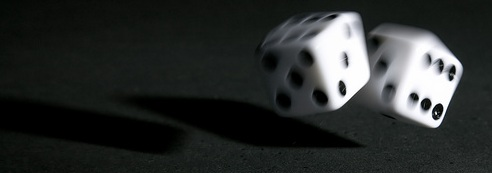
\includegraphics[width=3in]{dice.jpg}
\end{figure}
\FloatBarrier
}

\begin{enumerate}

\easysubproblem What brand name r.v. is $X_1$ distributed as? Write $X \sim$ something and make sure the parameters are correct.

\easysubproblem Does $X_1 \equalsindist X_2$? \spc{1}

\easysubproblem Are $X_1$ and $X_2$ independent? \spc{1}


\easysubproblem Find $\expe{X_i}$ for $i \in \braces{1,2}$ from first principles. \spc{2}

\easysubproblem Find $\var{X_i}$  for $i \in \braces{1,2}$ from first principles. \spc{2}

\easysubproblem The standard deviation is also called \qu{standard error} and it sometimes denoted \qu{SE.} Use your answer in (e) to find $\se{X_i}$  for $i \in \braces{1,2}$. Please just use the square root and do not rederive the variance again from scratch.  \spc{1}

\easysubproblem Draw the PMF for $X_i$  for $i \in \braces{1,2}$ and mark $\expe{X_i}$ and $\se{X_i}$ on the graph similar to how we did in class. \spc{4}

\easysubproblem Imagine the game where you just double the winnings of a single roll. This would be equivalent to just multiplying the r.v. by a scale factor of 2. Calculate $\expe{2X_i}$, $\var{2X_i}$ and $\se{2X_i}$ from the formulas we learned in class.  \spc{3}

\easysubproblem Draw the PMF for $2X_i$ for $i \in \braces{1,2}$ and mark $\expe{2X_i}$ and $\se{2X_i}$ that you calculated in (h) on the graph similar to how we did in class.  \spc{4}

\intermediatesubproblem Draw the PMF for $X_1 + X_2$. This involves taking a convolution. Since I don't want to focus on the convolution and it won't be on the midterm or final, I'm going to give a hint. There is 1 way to get 2 or 12, 2 ways to get 3 or 11, 3 ways to get 4 or 10, 4 ways to get 5 or 9, 5 ways to get 6 or 8 and 7 ways to get 7.  \spc{4}

\easysubproblem Calculate $\expe{X_1 + X_2}$, $\var{X_1 + X_2}$ and $\se{X_1 + X_2}$ from the formulas we learned in class.  \spc{2}

\hardsubproblem Why are the standard errors in (h) and (k) different and why is (h) larger? This involves a lot of thinking and I want a few sentences \textit{in English}.  \spc{3}

\intermediatesubproblem Imagine $n$ rolls of the same dice to produce $n$  r.v.'s denoted $X_1, \ldots, X_n$ which of course are still $\iid$. Calculate $\expe{X_1 + \ldots + X_n}$, $\var{X_1 + \ldots + X_n}$ and $\se{X_1 + \ldots + X_n}$.  \spc{2}

\intermediatesubproblem Calculate $\expe{\Xbar_n}$, $\var{\Xbar_n}$ and $\se{\Xbar_n}$ using the definition of $\Xbar_n$ we learned in class. Calculate means give the numeric answer, not leave in terms of $n$ and $\mu$ and whatnot. I know you can copy the formulas from my notes.  \spc{3}

\hardsubproblem What does it mean that $\expe{\Xbar_n}$ is an unbiased estimator for $\mu$? Read about unbiased estimators in the book or online. It is also touched on in my lecture but I went through it quickly.  \spc{3}

\easysubproblem If $n=1000$, what is $\se{\Xbar_n}$? Does that mean it's getting really close to $\expe{\Xbar_n}$? Why or why not. \spc{2}

\hardsubproblem Now you have the choice between game A --- where you roll $n$ times and average the winnings (\ie you collect $\Xbar_n$ dollars at the end) or game B --- where you roll one die and collect the amount you make on just one roll. Use your answers to the relevant previous questions (I won't tell you which ones explicitly) to explain why you would choose game A over B or vice versa. I want multiple sentences \textit{in English}. You must convince me you understand the tradeoff that game A and B are making. \spc{3}

\intermediatesubproblem Let $Z$ be the standardized r.v. for $\Xbar_n$. Prove from the formulas in class that $\expe{Z} = 0$ and $\var{Z} = \se{Z} = 1$. \spc{3}

\easysubproblem If $n=1000$ and you made $\xbar = \$4.00$, what is the $z$-score of this $\xbar$? That is if $\Xbar_n$ was standardized into the r.v. $Z$ (as in the previous question), what would be the corresponding realization of $z$ that corresponds to this $\xbar$. \spc{2}

\easysubproblem We will learn later in Math 241 that $z \notin \bracks{-3,3}$ are very strange and smack of something being awry. Is something awry with making \$4.00 on average? Explain using a sentence \textit{in English}.\spc{3}

\end{enumerate}

\problem More simple r.v. practice.

\begin{enumerate}

\hardsubproblem Let $T_n \sim \binomial{n}{p}$. Prove that $\var{T_n} =np(1-p)$ from first principles. This involved two reindexing tricks in the notes. \spc{9}

\intermediatesubproblem Let $X_1 \sim \bernoulli{p}$. Derive an expression for $\var{X_1}$ as a function of the parameter as we did in class.  \spc{3}

\easysubproblem You know that $T_n$ is the sum of $n$ $\iid$ bernoulli r.v.s with parameter $p$. Show that $\var{T_n}$ can be easily derived using the variance-sum formula we learned in class.  \spc{3}

\intermediatesubproblem If you had complete control of both parameters $n$ and $p$, what would be the easiest manipulation to make variance as small as possible?  \spc{1}

\easysubproblem In (d) and (e), in the limit of that manipulation, what would the final r.v. be? The name and how it's distributed is all that's needed ($X \sim$ somthing).  \spc{1}

\easysubproblem Prove $\var{X} = \expe{X^2} - \musq$ for any r.v. $X$.  \spc{3}

\easysubproblem Show from the definition of variance that $\var{X} \geq 0$ for any r.v. $X$.  \spc{2}

\hardsubproblem Find a r.v. $X$  where $\var{X} = 0$.  \spc{3}

\hardsubproblem Show for any two r.v.'s $X$ and $Y$ which are independent (you need the independence) that $\var{XY} = \musq_X \sigsq_Y + \musq_Y \sigsq_X + \sigsq_X \sigsq_Y$.  \spc{4}

\easysubproblem Let $a_1, a_2, \ldots, a_n$ be a sequence of constants. Let $X_1, \ldots, X_n$ be a sequence of r.v.'s which share the same mean. Create a simplified expression for $\expe{a_1 X_1 + \ldots + a_n X_n}$.  \spc{2}

\intermediatesubproblem Let $a_1, a_2, \ldots, a_n$ be a sequence of constants.  Assume $X_1, \ldots, X_n$ are a sequence of $\iid$ r.v.'s. Create a simplified expression for $\se{a_1 X_1 + \ldots + a_n X_n}$.  \spc{2}

\intermediatesubproblem Imagine a r.v. $X$ with density $f(x) = c/x^2$ and $\support{X} = \naturals$. What is the exact value of $c$ which makes $f(x)$ a valid PMF? The answer can be found \href{http://en.wikipedia.org/wiki/Riemann_zeta_function}{here}.  \spc{3}

\easysubproblem Show that $\expe{X^2}$ does not exist (which of course means by (f) that $\sigsq$ does not exist). This should be extremely easy from the definition of $\expe{g(X)}$ which we've done in class many times.  \spc{2}

\intermediatesubproblem Show that $\expe{X}$ does not exist. You will need a fact from that same wikipedia page that you visited in (m). And now you've learned what the harmonic series is too.  \spc{3}

\intermediatesubproblem Consider $X \sim \negbin{r}{p}$. Prove that $\var{X} = r(1-p)/p^2$ assuming that the variance of a geometric r.v. with parameter $p$ is $(1-p)/p^2$.


\end{enumerate}



\end{document}
%%%%%%%%%%%%%%%%%%%%%%%%%%%%%%%%%

\problem Queens Blvd. is known by some as the \qu{Boulevard of Death} (you can read the Wikipedia information \href{http://en.wikipedia.org/wiki/Queens_Boulevard#Boulevard_of_Death}{here}). 

\iftoggle{professormode}{
\begin{figure}[htp]
\centering
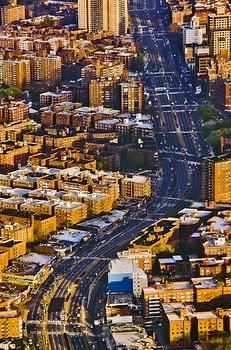
\includegraphics[width=2in]{qb.jpg}
\end{figure}
\FloatBarrier
}

From Wikipedia:

\begin{quotation}
\sf From 1993 to 2000, 72 pedestrians, were killed trying to cross the street, an average of 10 per year, with countless more injuries. Since 2000, at least partially in response to major news coverage of the dangerous road, the city government has taken measures to cut down on such incidents, including posting police along parts of the boulevard and doing spot-ticketing stings of jay-walkers against traffic, posting large signs proclaiming that ``A Pedestrian Was Killed Crossing Here'' at intersections where fatal accidents have occurred and installing more road-rule enforcement cameras.
\end{quotation}

Fatal pedestrian accidents on Queens Blvd. since 2001 is presented in the table below:

\begin{table}[htp]
\centering
\begin{tabular}{ccccccc}
2001 & 2002 & 2003 & 2004 & 2005 & 2006 & 2007 \\ \hline
4&2&5&1&2&2&1
\end{tabular}
\caption{Number of pedestrian accidents by year.}
\label{tab:qbacc}
\end{table}

\begin{enumerate}

\easysubproblem Consider one year: 2001. Estimate the number of pedestrian crossings of Queens Blvd. in 2001. For those of you who ever interview for anything in business consulting, this is a good exercise. Note that this estimate does not use any of the data above nor any tools from my class that I can think of. \spc{1}


\easysubproblem Based on your answer to (a) and the data in the first cell of Table~\ref{tab:qbacc}, estimate the probability of a pedestrian accident on one crossing. \spc{1}

\easysubproblem Considering the rather large answer in (a) and the rather small answer in (b), let $X$ be the r.v. for number of pedestrian accidents in 2001. How is $X$ distributed? What are its parameter(s)? I want the value of the parameter(s) not just a greek letter. \spc{1}

\intermediatesubproblem Write all the possible problems with the model you created in (c). Note: I will do something like this on the exam: build a model, tell me the problems with it, use the model.\spc{3}

\easysubproblem We will now go a step further, consider the data above to be $\iid$ draws from one distribution --- the distribution Poisson you created in (c). However, their parameters may now be different. Thus, the accidents for 2001 -- 2007 can be thought of as:

\beqn
X_{2001}, X_{2002}, \ldots, X_{2007} \iid f(x)  
\eeqn

where the $f(x)$ is the PMF of a model similar to the one you built in (c) but maybe not with the same $\lambda$ parameter. Let:

\beqn
\Xbar := \frac{X_{2001} + X_{2002} + \ldots + X_{2007}}{7}
\eeqn

Is $\xbar$, the sample average using the data in Table~\ref{tab:qbacc} a realization from the $\Xbar$ r.v.? Yes or no is fine.\spc{1}

\easysubproblem If we had many more years of data than the 7 years, what would $\Xbar$ converge to eventually? You can use notation and not answer using a number. \spc{1}

\easysubproblem What is the law we used in part (f)? Look in your notes. State the law and write a sentence about what it means to you \textit{in English}.\spc{3}

\easysubproblem Calculate $\xbar$, the sample average using the data in Table~\ref{tab:qbacc}. \spc{1}


\extracreditsubproblem This may seem like a non-sequitor, but we'll need it for the next problem. Prove from first principles (\ie from $\expe{X} := \sum_{x \in \support{X}} x f(x)$, the definition of expectation) that if $X \sim \poisson{\lambda}$ then $\expe{X} = \lambda$. \spc{10}

\easysubproblem Using the fact that $\expe{X} = \lambda$ if $X \sim \poisson{\lambda}$, pretend 7 years of data is as good as infinite years of data and use your answer to (h) to approximate $\lambda$ by setting $\lambda = \xbar$. Now, build a general model for number of annual pedestrian accidents. \qu{$X \sim$ something} is all you need to write below. \spc{4}

\intermediatesubproblem Fill in the following table for the r.v. X you built in (j). Use three decimal places ONLY. (That goes \textbf{double }for Ilya, Joe and others). If you are feeling really lazy, check out \qu{\texttt{dpois(0:8, ---)}} and \qu{\texttt{ppois(0:8, ---)}} in \texttt{R} where the dash is your answer to (h).

\begin{table}[h]
\centering
\Large
\begin{tabular}{c|c|c}
$x$ & $~~~~f(x)~~~~$ & $~~~~F(x)~~~~$ \\ \hline
0 && \\
1 && \\ \hline
2 && \\
3 && \\ \hline
4 && \\
5 && \\ \hline
6 && \\
7 && \\ \hline
8 && \\
\end{tabular}
\end{table}
\FloatBarrier

\easysubproblem Find the $\quantile{X}{0.10}$.\spc{1}

\easysubproblem Find the 99\%ile of $X$.\spc{1}

\easysubproblem Find the $\median{X}$.\spc{1}

\easysubproblem Find the $\IQR{X}$.\spc{1}

\easysubproblem Find the $\mode{X}$.\spc{1}

\easysubproblem Estimate the $\prob{X > 8}$ based on your calculation of $F(8)$.\spc{1}

\easysubproblem Is it fair to say for a few draws of $X$ the support essentially is just $\braces{0, \ldots, 8}$? Write yes/no plus a sentence explanation.\spc{1}

\hardsubproblem What is the probability in 100 years of data you see more than 1 year with the number of pedestrian accidents greater than 8?\spc{3}

\hardsubproblem This is a preview of what's to come when we get to Statistics. Consider the hypothetical scenario where Queens Borough President Melinda Katz institutes new safety precautions for Queens Blvd. In 2015, the number of accidents drop to 0. Based on the table you completed in (k), can you say with assurance that this drop was due to President Katz's efforts? Why or why not? Justify using a number and a sentence \textit{in English}.\spc{4}

\end{enumerate}



\problem We are going to return to our in-class discussion of the my ride from my office to my apartment in Forest Hills using the Uber Taxi service. Since Queens is in New York City, I will be modeling based on Uber NYC rates. The current rates are posted \href{https://www.uber.com/en-US/cities/new-york}{here}. I have extra incentive now to provide you with a realistic model. Thanks for helping me plan my budget!

\iftoggle{professormode}{
\begin{figure}[htp]
\centering
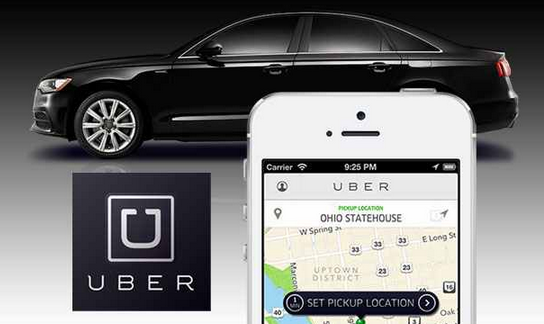
\includegraphics[width=2.5in]{uber.png}
\end{figure}
\FloatBarrier
}

For the purposes of this exercise, assume there are only two routes in which to drive back. This is close to realistic. There is the \qu{Van Wyck} (outlined in black on the right below) and \qu{Jewel Ave} which is the Q64 bus route (outlined in black on the left below).

\iftoggle{professormode}{
\begin{figure}[htp]
\centering
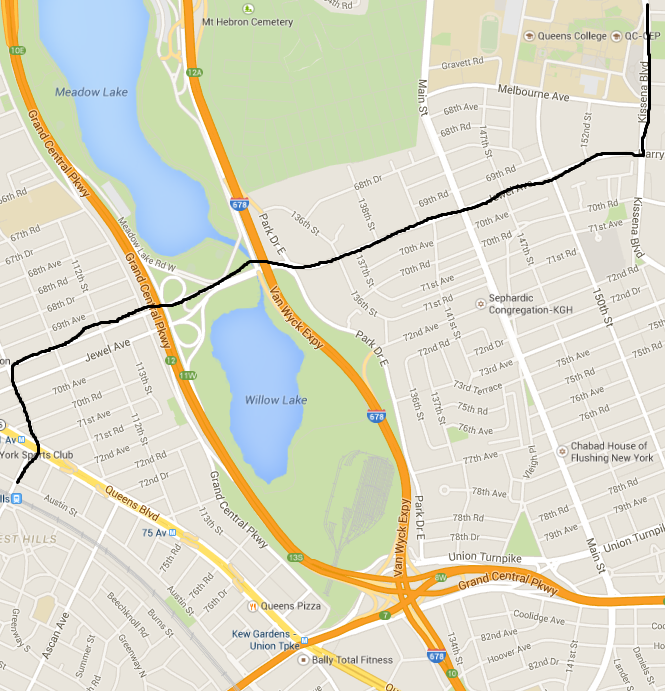
\includegraphics[width=3in]{route1.png}~~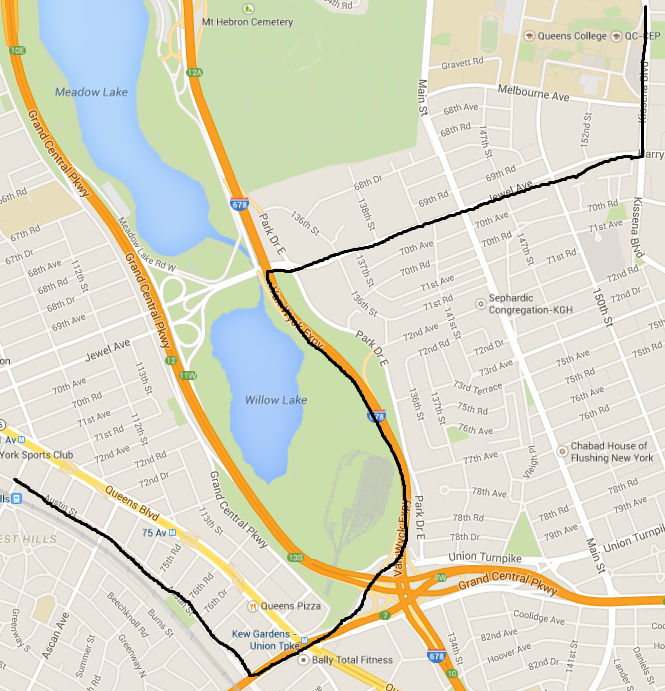
\includegraphics[width=3in]{route2.png}
\end{figure}
\FloatBarrier
}

The only determinant of route selection is whether or not there is traffic on the Van Wyck. If there is traffic, I take Jewel Ave route; if not, I take the Van Wyck route. The probability of traffic on the Van Wyck is 30\%. The Jewel Ave route is 2.3 miles and takes 10 min and the Van Wyck route is 6 min and is 3.6 miles.

\begin{enumerate}
\easysubproblem Let $W$ be the r.v. which models the time I travel in the Uber Taxi. What is its distribution? Use the notation we used in class.\spc{2}

\easysubproblem What is $\support{W}$?\spc{1}

\easysubproblem Compute $\expe{W}$ from the definition of expectation.\spc{2}

\easysubproblem Write a sentence that synthesizes what part (c) means.\spc{1}

\easysubproblem Let $D$ be the r.v. which models the distance I travel in the Uber Taxi. What is its distribution? Use the notation we used in class.\spc{2}

\easysubproblem Compute $\expe{D}$.\spc{2}

\hardsubproblem Are the r.v.'s $W$ and $D$ dependent? Justify your answer \textit{in English}.\spc{3}

\easysubproblem Write a sentence that synthesizes what part (f) means.\spc{1}

\easysubproblem UberX charges \$0.40\textbackslash min. Let $M$ be the r.v. which is what I pay for time on my trip home. Find the distribution of $M$.\spc{2}

\easysubproblem Write $M$ as a function of $W$.\spc{1}

\easysubproblem Calculate $\expe{M}$ based on the formula we learned in class about expectations of r.v.'s scaled by a constant.\spc{1}

\easysubproblem UberX charges \$2.15\textbackslash mi of distance covered. Let $L$ be the r.v. which is what I pay for mileage on my trip home. Find the distribution of $L$.\spc{2}

\easysubproblem Write $L$ as a function of $D$.\spc{1}

\easysubproblem Calculate $\expe{L}$ based on the formula we learned in class about expectations of r.v.'s scaled by a constant.\spc{1}

\easysubproblem Uber also includes a base fare of \$3. Let $B$ be the r.v. which models the total bill for my uberX ride. Write $B$ as a function of $W$ and $D$.\spc{1}

\intermediatesubproblem We didn't really cover this in class, but you should be able to do it. $W$ and $D$ are one-to-one so the scaled $W$ and scaled $D$ sum is really one r.v. Find $\expe{B}$ based also on the formula we learned in class about the expectation of a r.v. with a constant added. \spc{4}

\easysubproblem Write a sentence that synthesizes what part (p) means.\spc{1}

\hardsubproblem UberBLACK is the original Uber taxi service. They dispatch a luxury black sedan to pick me up. The base fare is \$7 and they charge \$0.65\textbackslash min and \$3.75\textbackslash mi. Calculate $\expe{B}$ where $B$ is now the total bill for UberBLACK.\spc{3}

\intermediatesubproblem UberSUV dispatches an SUV and it is particularly useful if I'm transporting stuff between my office and apartment. The base fare is \$14 and they charge \$0.80\textbackslash min and \$4.50\textbackslash mi. Calculate $\expe{B}$ where $B$ is now the total bill for UberSUV.\spc{3}

\end{enumerate}

\problem This is the fun part of the homework. You're going to repeat the experiments we did in class. 

\iftoggle{professormode}{
\begin{figure}[htp]
\centering
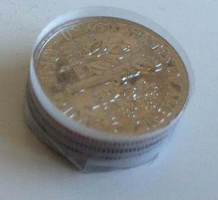
\includegraphics[width=1.3in]{coins.png}
\end{figure}
\FloatBarrier
}

\begin{enumerate}
\easysubproblem Write the definitions of \qu{datum} and \qu{data.} \spc{2}

\easysubproblem Why are r.v.'s also called \qu{data generating processes?} \spc{2}

\easysubproblem Grab a cup and 8 pennies (or nickels, or dimes, etc). Use a magic marker to mark four of them (front and back). If you shake the cup and pull out three coins, let $X$ be the r.v. for how many marked coins you pull out? How is $X$ distributed? Write \qu{$X \sim$ something} below.\spc{1}

\extracreditsubproblem For $X \sim \hypergeometric{n}{K}{N}$, show that $\expe{X} = n\frac{K}{N}$ from first principles  (\ie from $\expe{X} := \sum_{x \in \support{X}} x f(x)$, the definition of expectation). This is hard...\spc{12}

\easysubproblem Using as fact that $\expe{X} = n\frac{K}{N}$ when  $X \sim \hypergeometric{n}{K}{N}$, calculate $\expe{X}$ for the r.v. you constructed in part (c). \spc{3}

\easysubproblem Shake the cup and take out 3 coins. How many were marked? Repeat this five times. 
Record your data below. That is, just write down the five numbers separated by commas.\spc{1}

\easysubproblem Find $\xbar$ from the data you recorded in part (e). \spc{1}

\easysubproblem Is $\xbar \approx \expe{X}$? If not, what could you change in the experiment to make $\xbar$ closer to $\expe{X}$? \spc{1}

\easysubproblem Now forget that the coins are marked. If you shake the cup and flip all 8 coins, let $X$ be the r.v. for how many heads are flipped. How is $X$ distributed? Write \qu{$X \sim$ something} below.\spc{1}

\hardsubproblem For $X \sim \binomial{n}{p}$, show that $\expe{X} = np$ from first principles  (\ie from $\expe{X} := \sum_{x \in \support{X}} x f(x)$, the definition of expectation). Try to do this yourself and if you give up, you can copy this fron your notes.\spc{10}

\easysubproblem Using as fact that $\expe{X} = np$ when  $X \sim \binomial{n}{p}$, calculate $\expe{X}$ for the r.v. you constructed in part (i). \spc{1}

\easysubproblem Shake the cup and count the number of heads. Repeat this five times. 
Record your data below. \spc{1}

\easysubproblem Find $\xbar$ from the data you recorded in part (l).  \spc{1}

\easysubproblem Is $\xbar \approx \expe{X}$? If not, what could you change in the experiment to make $\xbar$ closer to $\expe{X}$? \spc{1}


\easysubproblem Now imagine one coin in the cup and success is defined as getting a head. Further imagine that you don't stop flipping this coin until you get a head. Let $X$ be the r.v. for how many flips you make. How is $X$ distributed? Write \qu{$X \sim$ something} below. \spc{1}

\extracreditsubproblem For $X \sim \geometric{p}$, show that $\expe{X} = 1/p$ from first principles  (\ie from $\expe{X} := \sum_{x \in \support{X}} x f(x)$, the definition of expectation).  \spc{11}

\easysubproblem Using as fact that $\expe{X} = 1/p$ when  $X \sim \geometric{p}$, calculate $\expe{X}$ for the r.v. you constructed in part (o). \spc{1}

\easysubproblem Flip until you get a head. Repeat this five times. Record your data below. \spc{1}

\easysubproblem Find $\xbar$ from the data you recorded in part (r).  \spc{1}

\easysubproblem Is $\xbar \approx \expe{X}$? If not, what could you change in the experiment to make $\xbar$ closer to $\expe{X}$? \spc{1}

\easysubproblem Now imagine one coin in the cup and success is defined as getting a head. Further imagine that you don't stop flipping this coin until you get two heads on at least two independent tosses. Let $X$ be the r.v. for how many flips you make. How is $X$ distributed? Write \qu{$X \sim$ something} below. \spc{1}

\extracreditsubproblem For $X \sim \negbin{r}{p}$, show that $\expe{X} = r/p$ from first principles  (\ie from $\expe{X} := \sum_{x \in \support{X}} x f(x)$, the definition of expectation). You need to use a trick. It is related to the trick from last week's extra credit problem. \spc{11}

\easysubproblem Using as fact that $\expe{X} = r/p$ when $X \sim \negbin{r}{p}$, calculate $\expe{X}$ for the r.v. you constructed in part (u). \spc{1}

\easysubproblem Flip until you get two heads. Repeat this five times. Record your data below. \spc{1}

\easysubproblem Find $\xbar$ from the data you recorded in part (x).  \spc{1}

\easysubproblem Is $\xbar \approx \expe{X}$? If not, what could you change in the experiment to make $\xbar$ closer to $\expe{X}$? Note: I tried to make another question, but \LaTeX ~crashed after (z).\spc{1}
 
\end{enumerate}


\end{document}
